\documentclass[11pt]{article}
\usepackage{amssymb}
\usepackage{dsfont}
\usepackage{amsmath}
\usepackage{amssymb}
\usepackage[utf8]{inputenc}
\usepackage{ dsfont }
\usepackage{enumitem}
\usepackage{titlesec}
\usepackage{tocloft}
\usepackage{hyperref}
\hypersetup{
    colorlinks=true,
    linkcolor=black,
    filecolor=magenta,      
    urlcolor=blue,
    pdftitle={notes},
    pdfpagemode=FullScreen,
    }
\usepackage{lmodern}
\usepackage{fancyhdr}
\usepackage{xcolor}
\usepackage{geometry}
\usepackage{array}
\usepackage{enumitem}
\usepackage{mathtools}
\geometry{margin=1in}
\usepackage{tikz}
\usepackage{tikz-qtree}
\usepackage{float}
\usetikzlibrary{arrows,automata,positioning,shadows}
\usepackage[many]{tcolorbox}
\setlength{\parindent}{0pt}

\tikzset{
	->, % makes the edges directed
	shorten >=1pt,
	shorten <=1pt,
	node distance=2cm,
	on grid,
	>=stealth', % makes the arrow heads bold
	thick,
	initial text = {},
	every state/.style={thin, fill=red!30},	
	accepting/.style ={ultra thick,fill=green!30},
}


% TOC formatting
\renewcommand{\cftsecfont}{\bfseries}
\renewcommand{\cftsecpagefont}{\bfseries}


\newcommand{\defn}[0]{\tcbhighmath[boxrule=0.5mm, colframe=cyan!20, colback=cyan!20, arc=10mm, size=fbox]{\textbf{DEF:}}}
\newcommand{\ex}[0]{\tcbhighmath[boxrule=0.5mm, colframe=pink, colback=pink, arc=10mm, size=fbox]{\textbf{Ex:}}}
\newcommand{\thm}[0]{\tcbhighmath[boxrule=0.5mm, colframe=orange!20, colback=orange!20, arc=10mm, size=fbox]{\textbf{Thm:}}}
\newcommand{\prop}[0]{\tcbhighmath[boxrule=0.5mm, colframe=orange!20, colback=orange!20, arc=10mm, size=fbox]{\textbf{Prop:}}}
\newcommand{\N}{\mathbb{N}}
\newcommand{\R}{\mathbb{R}}
\newcommand{\ru}[1]{\textcolor{red}{\underline{#1}}}

\newcommand{\subsubsubsection}[1]{%
  \vspace{1em}%
  \noindent\textit{#1}%
  \vspace{0.5em}%
  \par%
}

\newcommand{\pf}{\textit{Proof. }}

\begin{document}
% Custom title layout
\begin{center}
    {\LARGE \textbf{Theory of Computation}} \\[0.5em]
    {\large Claire Driedger} \\[0.3em]
    {\normalsize Feb-June, 2025}
\end{center}
\noindent
\colorbox{gray!20}{%
  \parbox{\textwidth}{%
    References: Lectures by Stephen Cranefield in COSC341 at the University of Otago, New Zealand; Lecture Slides mostly by Michael Albert; \href{https://www3.nd.edu/~kogge/courses/cse30151-fa17/Public/other/tikz_tutorial.pdf}{tikz tutorial} by Satyaki Sikdar
  }
}

\tableofcontents
\newpage

\section{Deterministic Finite State Automaton (DFAs)}

\subsection{Introduction to DFAs}

\defn  A \textit{deterministic finite state automaton (DFA)}, \textbf{A}, consists of the following:
\begin{itemize}[itemsep=-2pt]\setlength{\baselineskip}{10pt}
  \hangindent=2em  
    \item A finite set $\Sigma$ called its \textcolor{red}{\underline{alphabet}}, \\ 
    \hspace{20em} \footnotesize{ the \textit{alphabet} can be thought of as keys on the keyboard, or events}
    \item \normalsize{A finite set $\mathcal{S}$ called its \textcolor{red}{\underline{states}}},\\
    \hspace{20em} \footnotesize{the \textit{states} can be thought of as symbols without meaning}
    \item \normalsize{A function $T :\mathcal{S} \times \Sigma \to \mathcal{S}$ called its \textcolor{red}{\underline{transition function}},}\\
    \hspace{20em} \footnotesize{the \textit{transition function} takes as input the current state and a letter from the alphabet}
    \item \normalsize{A single element $s \in \mathcal{S}$ called its \textcolor{red}{\underline{start state}},}
    \item \normalsize{A subset $A \subseteq \mathcal{S}$ called its \textcolor{red}{\underline{final states}} or \textcolor{red}{\underline{accepting states}}.}
\end{itemize}
\textit{Notes:} 
\begin{itemize}[itemsep=-2pt]\setlength{\baselineskip}{10pt}
  \item Changes to the state of any model always occur sequentially, not in parallel.
  \item The DFA has a limited, finite memory, and no history
\end{itemize}


We begin with an example. Consider a light with two switches. Flipping either switch changes the state of the light.\\

\quad\quad \ex 
\begin{figure}[ht] % ’ht’ tells LaTeX to place the figure ’here’ or at the top of the page
\centering % centers the figure
    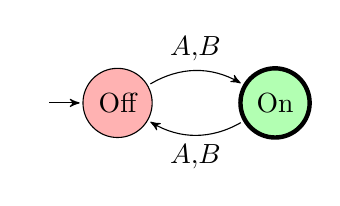
\begin{tikzpicture}
    
    \node[state, initial] (Off) {Off};
    \node[state, accepting, right of=Off] (On) {On};
    
    \draw (Off) edge[bend left, above] node{$A,\!B$} (On);
    \draw (On) edge[bend left, below] node{$A,\!B$} (Off);

\end{tikzpicture}
\caption{Two buttons, one light}
\label{fig:2b1l}
\end{figure}

\begin{itemize}[itemsep=-2pt]\setlength{\baselineskip}{10pt}
  \item The light starts in the \textbf{Off} state. 
  \item In either state, making an input of either \textit{A} or \textit{B} switches to the other state. 
  \item We consider the \textbf{On} state to be \textit{accepting} -- any sequence of inputs that leads to this state is considered successful
  \item The successful inputs are all strings consisting of characters from ${A, B}$ that have an \underbar{odd number of characters}.
\end{itemize}

\quad\quad \ex
\begin{figure}[H] % ’ht’ tells LaTeX to place the figure ’here’ or at the top of the page
  \centering % centers the figure
      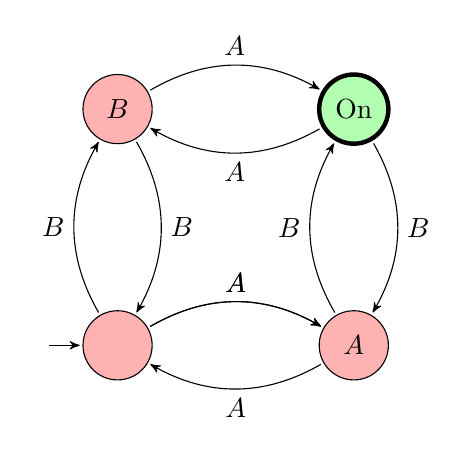
\begin{tikzpicture}[node distance=3cm]
      
      \node[state, initial] (Off) {};
      \node[state, right of=Off] (A) {$A$};
      \node[state, above of=Off] (B) {$B$};
      \node[state, accepting, right of=B] (On) {On};
      
      \draw (Off) edge[bend left, left] node{$B$} (B);
      \draw (B) edge[bend left, right] node{$B$} (Off);
      
      \draw (Off) edge[bend left, above] node{$A$} (A);
      \draw (A) edge[bend left, below] node{$A$} (Off);
      \draw (Off) edge[bend left, above] node{$A$} (A);
      
      \draw (On) edge[bend left, right] node{$B$} (A);
      \draw (A) edge[bend left, left] node{$B$} (On);

      \draw (B) edge[bend left, above] node{$A$} (On);
      \draw (On) edge[bend left, below] node{$A$} (B);
    \end{tikzpicture}
  \caption{Two different buttons, one light}
  \label{fig:2b1l}
  \end{figure}

\begin{itemize}[itemsep=-2pt]\setlength{\baselineskip}{10pt}
  \item The light starts in the lower left state. 
  \item The successful inputs are all strings consisting of characters from $\{A, B\}$ that have an \underbar{odd number of each letter}.  
\end{itemize}

\quad\quad \ex \quad What does this machine do?

\begin{center}
	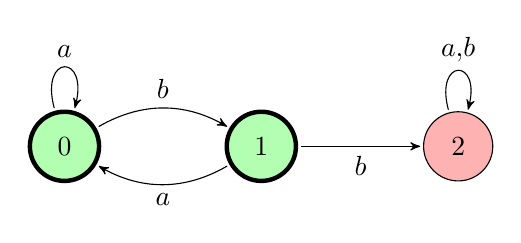
\begin{tikzpicture}
	\node[state, accepting] (0) at (0,0) {$0$};	
	\node[state, accepting] (1)  at (2.5,0) {$1$};
	\node[state] (2) at (5,0) {$2$};
	
	\draw 	(0) edge[loop above] 						        node{$a$} (0)
					(0) edge[bend left, above]							node{$b$} (1)
          (1) edge[bend left, below]              node{$a$} (0)
					(1) edge[below]								          node{$b$} (2)
					(2) edge[loop above]						        node{$a,\!b$} (2);					
  \end{tikzpicture}
\end{center}

\begin{itemize}[itemsep=-2pt]\setlength{\baselineskip}{10pt}
  \item The machine starts in the \textcolor{red}{\underbar{state}} labelled 0.
  \item There are two buttons to press - \textit{a} and \textit{b}. These define the \textcolor{red}{\underbar{alphabet}} of the machine.
  \item Each button press causes a \textcolor{red}{\underbar{transition}} according to the labelled arrows.
  \item The sequence of button presses leaving us in an \textcolor{red}{\underbar{accepting state}} (coloured green) are the \textcolor{red}{\underbar{language}} accepted by the machine.
\end{itemize}

\quad\quad \ex 

\begin{figure}[ht] % ’ht’ tells LaTeX to place the figure ’here’ or at the top of the page
  \centering % centers the figure
      \begin{tikzpicture}[node distance=2cm]
      
      \node[state, initial] (Off) {0};
      \node[state, accepting, right of=0] (1) {1};
      \node[state, right of=1] (2) {2};

      \draw (0) edge[loop above] node{$A$} (0);
      \draw (0) edge[above] node{$B$} (1);

      \draw (1) edge[above] node{$A,\!B$} (2);

      \draw (2) edge[loop above] node{$A, \!B$} (2);  
  \end{tikzpicture}
  \label{fig:2b1l}
  \end{figure}

In this example, the accepted language is exactly ``zero or more copies of A followed by exactly one B".

\subsection{Automata and Grammars}

\defn A \textit{sequence of length $n$ over $\Sigma$} is a function:
$$
\sigma: \{ 0, 1, 2, \dots, n-1\} \to \Sigma.\\
$$
\centerline{\small{the function takes as input the subscript and outputs an element of the alphabet}}\\

\normalsize{} When $n=0$, we denote the empty string $\epsilon$.\\
The set of all strings over $\Sigma$ is denoted $\Sigma ^*$.\\

\defn A \textit{string of length $n$ over $\Sigma$} is a sequence $\sigma_0 \sigma_1 \dots \sigma_{n-1}$ where each $\sigma_i \in \Sigma$.\\
This is an \textit{array-like} definition of a string. With this definition, we can consider the concatenation of two strings, for example,
$$
``black'' + ``dog'' \to ``blackdog''
$$
With the indexing of $``blackdog"$ as $w_0 \dots w_{n-1} v_0 ... v_{k-1}$ given by the following $\sigma$ function:
$$
c(i) = \begin{cases} 
      w(i) & i < n \\
      v(i-n) & i \geq n 
   \end{cases}
$$

On the other hand, the recursive definition  of a string involves composing an element with the previous string.
Formally, this involves:
\begin{enumerate}
  \item Base case: The empty string, $\epsilon$
  \item Recursive step: A pair $(x, s)$, where $x \in \Sigma$ and $s$ is a string over $\Sigma$
\end{enumerate}
We can similarly define the length of a string recursively by
\begin{enumerate}
  \item Base case: $len(\epsilon) = 0$
  \item Recursive step: $len((x, s)) = 1 + len(s)$
\end{enumerate}

\defn The \textit{language accepted by \textbf{A}}, $L(\textbf{A})$ is the set of all strings over $\Sigma$ such that ``when you press the buttons defined by the string you wind up in an accepting state".\\

\ex What is the language accepted by the following machine?
\begin{center}
	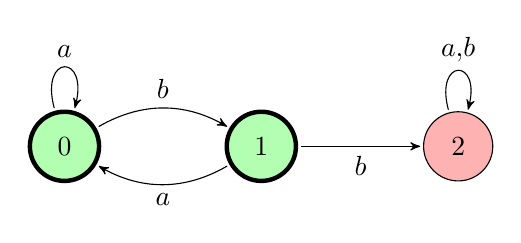
\begin{tikzpicture}
	\node[state, accepting] (0) at (0,0) {$0$};	
	\node[state, accepting] (1)  at (2.5,0) {$1$};
	\node[state] (2) at (5,0) {$2$};
	
	\draw 	(0) edge[loop above] 						        node{$a$} (0)
					(0) edge[bend left, above]							node{$b$} (1)
          (1) edge[bend left, below]              node{$a$} (0)
					(1) edge[below]								          node{$b$} (2)
					(2) edge[loop above]						        node{$a,\!b$} (2);					
  \end{tikzpicture}
\end{center}

We begin by listing all strings using formal grammar production rules in text form: $\text{start state} \to \text{accepting strings}$:
$$
\begin{aligned}
  S_0 &\to \epsilon \mid a S_0 \mid b S_1 \\
  S_1 &\to \epsilon \mid a S_0 \mid b S_2 \\
  S_2 &\to a S_2 \mid b S_2
\end{aligned}
$$
\textit{$\epsilon$ is included as a valid transition for $S_0$ and $S_1$ because these are already accepting states. However, $S_2$ is not an accepting state, so $\epsilon$ is not included as a transition state.}\\

The idea is to think about for each state $X$ (and not only the DFA’s start state) all the strings that you could accept starting from $X$.
A transition $T(S, a) = B$ in the DFA tells us that one way
to accept a string (if we were allowed to start with state $S$) is to receive an $a$ and then accept a string \textit{starting from $B$}.
That leads to the grammar production rule $S \to a B$.\\
Each state in the DFA corresponds to a non-terminal symbol in the grammar.\\\\
The language accepted by the machine is:
$$
\begin{aligned}
  S &\to \epsilon \mid a S \mid b B \\
  B &\to \epsilon \mid a S
\end{aligned}
$$

\subsubsection{Regular grammars}

\defn A \ru{right-regular grammar}, $G$, consists of:
\begin{itemize}[itemsep=-2pt]\setlength{\baselineskip}{10pt}
  \item An \ru{alphabet}, $\Sigma$, (\{$a, b$\}).
  \item A set $N$ of \ru{non-terminal symbols}, (\{$S, B$\}) (the \textit{states})
  \item A designated \ru{start symbol}, $S \in N$
  \item A list of \ru{production rules} ($S \to aS$) each of one of the forms:
    \begin{itemize}[itemsep=-2pt]\setlength{\baselineskip}{10pt}
      \item $X \to \epsilon$ ($X \in N$)
      \item $X \to a$ ($X \in N$, $a \in \Sigma$)
      \item $X \to aY$ ($X, Y \in N$, $a \in \Sigma$) 
    \end{itemize}
\end{itemize}

Note the recursive nature of the production rules. Events from the language are `terminal' and states are 'non-terminal'. To generate the language, we continue applying production rules until there are no non-terminal symbols left.\\
We might ask: ``are the accepting states of the DFA the same as the language generated by a right-regular grammar?''

\subsubsection{From grammar to language}

Each non-terminal, $X$ of a regular grammar, $G$, has an associated \ru{language}, $L_G(X)$ (or $L(X)$) which is a subset of $\Sigma ^*$ defined recursively as follows:
  \begin{enumerate}
    \item If $X \to \epsilon \in G$, then $\epsilon \in L(X)$, and if $X \to a \in G$, then $a \in L(X)$.
    \item For every production $X \to aY$ in $G$, $L(X)$ contains the set $aL(Y)$, meaning whatever can be generated from the new state $Y$.
  \end{enumerate}


When we say ``defined recursively'', we implicitely say ``and no other strings except those which must belong to $L(X)$ according to these rules are included''.\\

The language of the grammar itself is the language of its start state, $S$.\\

\ex Consider the right-regular grammar $G$ defined as follows:
$$
\begin{aligned}
  S &\to \epsilon \mid a S \mid b B \\
  B &\to \epsilon \mid a S
\end{aligned}
$$
\small{}\textit{This means, for example, that `a' followed by anything in the language for S is in the language.}\\  
\normalsize{}
We can build the language $L(S)$ (generated by $S$) and $L(B)$ (generated by $B$) from the bottom up:
\begin{itemize}[itemsep=-2pt]\setlength{\baselineskip}{10pt}
  \item $L(S)$ $=$ \textcolor{orange}{$\epsilon$}, \textcolor{blue}{$a$} ($a$ $+$ \textcolor{orange}{$\epsilon$}), \textcolor{green}{$b$} \text{ ($b$ $+$ \textcolor{orange}{$\epsilon$})}, \textcolor{yellow}{$aa$} \text{ ($a$ $+$ \textcolor{blue}{$a$})}, $ab$ ($a$ $+$ \textcolor{green}{$b$}), $b \textcolor{blue}{a}$, $\dots$
  \item $L(B)$ $=$ $\epsilon$, \textcolor{red}{$a$}, ($a$ $+$ \textcolor{orange}{$\epsilon$}), $a \textcolor{blue}{a}$, $a \textcolor{green}{b}$, $a$ $+$ \textcolor{yellow}{$aa$}, $aab$, $aba$, $\dots$
\end{itemize}
Characters are added on the left, rather than the right. \\

\textbf{Things which might be allowed in a regular grammar that are not allowed in a DFA:}
\begin{enumerate}
  \item Having multiple production rules with the same initial symbol
  $$
  A \to aB \mid aC \mid bD
  $$
  because at most one arrow leaves a node for each element of the alphabet
  \item Have no production rule with some initial symbol
  $$
  B \to \epsilon \mid aS
  $$
  because we need to consider at least one state for each letter of the alphabet.
\end{enumerate}
In a DFA, each state is supposed to have exactly one outgoing arrow corresponding to each letter of the alphabet.
\\ Do regular grammars potentially allow for \textit{more languages} than are represented by DFAs?


\subsection{Uncomputability}
\thm No reasonable model of computation allows \textbf{every} language to be recognized.\\

\pf{} 
Programs: $p_1, p_2, p_3, \dots$ (a sequence of programs) \\
Languages: $l1, l2, l3, \dots$ (a sequence of languages) \\
We will show that there exists a language $l = \dots $ s.t. $L \neq l_i$ for any $i$
Diagonalization proof:
   s1      s2     s3
l1 $\in$  $\notin$
l2       $\in$ 
                $\notin$
      
many languages will be the empty languages because it is syntactially incorrect
string 1 is either in L1 or not. 
Construct our new language with the diagonal: this language is new, and does not correspond to any language produced by our machines 
we enumerated all the possible machines: index all the languages they recognize

\section{Tutorials}
\subsection{Tutorial 01}
For this tutorial, the language $\Sigma = \{a, b \}$ is to be used throughout.
\begin{enumerate}
  \item \textit{How many different DFAs are there having only one state? What languages do they accept?} \\
  $\to$ There are exactly two DFAs having only one state (such a state is the start state and both transitions must loop on that state.) The only choice is whether or 
  not it is an accepting state. If the start is an accepting state, it accepts all strings (i.e. its language is $\Sigma ^*$), while the one where it is not accepting accepts
  no strings at all (i.e. it's language is \{\}, which does not even include the empty string).

\begin{minipage}{0.45\textwidth}
    \centering
    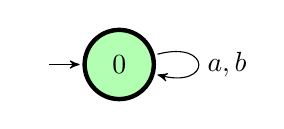
\begin{tikzpicture}
        \node[state, initial, accepting] (0)  {$0$};	
        \draw (0) edge[loop right] node{$a, b$} (0);				
    \end{tikzpicture}\\
    $L(A) = \Sigma ^*$
\end{minipage}
\hfill
\begin{minipage}{0.45\textwidth}
    \centering
    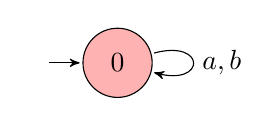
\begin{tikzpicture}
        \node[state, initial] (0)  {$0$};	
        \draw (0) edge[loop right] node{$a, b$} (0);				
    \end{tikzpicture}\\
    $L(A) = \{\}$
\end{minipage}

  \item \textit{A state in a DFA is \textit{unreachable} if there is no input sequence that leads to that DFA. Note that the start state is always reachable
  since the empty sequence $\epsilon$ leads to it. If we remove the unreachable states from a DFA how does that affect the language it accepts?} \\
  $\to$ Since a DFA can never enter an unreachable state, removing unreachable states does not affect the strings accepted by the DFA.

  \item \textit{How many different DFAs are there having only two states? What languages do they accept? Are they all different?} \\
  $\to$ Let the two states of such a DFA be 0 and 1. Which states are accepting and what are the transitions?
  \begin{enumerate}
    \item There are two choices of accepting/not-accepting for each of the two states.
    \item For each transition, there are two choices for its endpoint. There are two transitions for each of the two states.
  \end{enumerate}
  Therefore, we have six binary choices to make and the number of two-state DFAs is 
  $$
  2 \times 2 \times 2 \times 2 \times 2 \times 2 = 2^6 = 64
  $$
  In general, a DFA with $k$ states and an alphabet of size $n$ has $k$ binary state choices (accepting or not) and $kn$ transitions to choose endpoints for, each one having $k$ possibilities, generating
  $$
   2^k \times k^{kn}
  $$
  possible $k-state$ DFAs.\\
  For the accepting lanauge for the the two-state DFA:
  \begin{itemize}
    \item If both states are accepting, the language is $\Sigma ^*$
    \item If both states are non-accepting, the language is $\{\}$
  \end{itemize}
  This accounts for 32 DFAs. For the remaining 32 DFAs, one state is accepting and the other is not, and interchanging the states complements the accepting language.
  Consider the DFAs in which the start state is accepting and the other state isn't:
  \begin{center}
    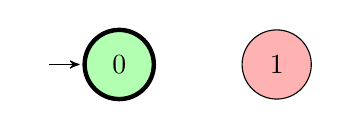
\begin{tikzpicture}
    \node[state, initial, accepting] (0)  {$0$};	
    \node[state, right of=0] (1)   {$1$};					
    \end{tikzpicture}
  \end{center}
  \begin{itemize}
    \item There are four DFAs in which $a$ and $b$ loop on the start state (the four are generated by the four transition states for $a$ and $b$ from $1$). The accepting language is $\Sigma^*$.
      \begin{center}
      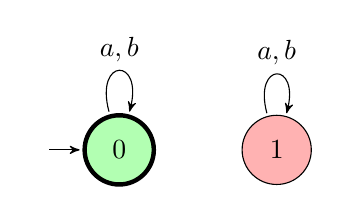
\begin{tikzpicture}
      \node[state, initial, accepting] (0)  {$0$};	
      \node[state, right of=0] (1)   {$1$};					
      
      \draw (0) edge[loop above]  node{$a, b$} (0);
      \draw (1) edge[loop above] node{$a, b$}   (1);
    \end{tikzpicture}
    \end{center}
    
    \begin{center}
      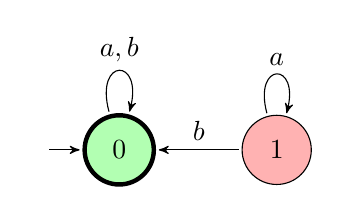
\begin{tikzpicture}
      \node[state, initial, accepting] (0)  {$0$};	
      \node[state, right of=0] (1)   {$1$};					
      
      \draw (0) edge[loop above]  node{$a, b$} (0);
      \draw (1) edge[loop above] node{$a$}   (1);
      \draw (1) edge[above]            node{$b$}   (0);
    
    \end{tikzpicture}
    \end{center}

    \begin{center}
      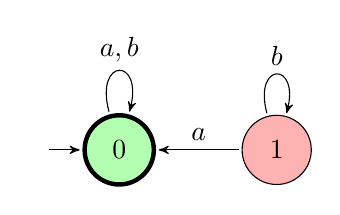
\begin{tikzpicture}
      \node[state, initial, accepting] (0)  {$0$};	
      \node[state, right of=0] (1)   {$1$};					
      
      \draw (0) edge[loop above]  node{$a, b$} (0);
      \draw (1) edge[loop above] node{$b$}   (1);
      \draw (1) edge[above]            node{$a$}   (0);
    
    \end{tikzpicture}
    \end{center}

    \begin{center}
      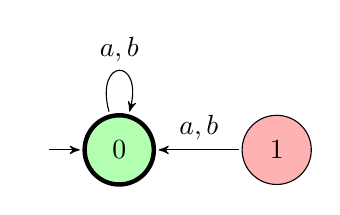
\begin{tikzpicture}
      \node[state, initial, accepting] (0)  {$0$};	
      \node[state, right of=0] (1)   {$1$};					
      
      \draw (0) edge[loop above]  node{$a, b$} (0);
      \draw (1) edge[above]            node{$a, b$}   (0);
    
    \end{tikzpicture}
    \end{center}

    \item If $a$ loops and $b$ transitions, it remains to consider the transitions from state 1:
    \begin{center}
      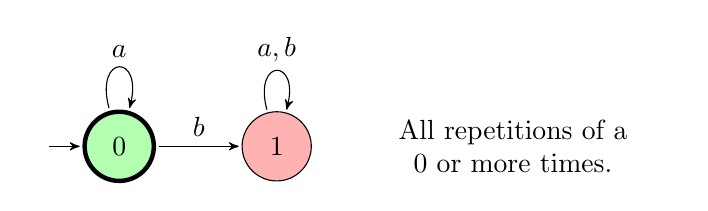
\begin{tikzpicture}
      \node[state, initial, accepting] (0)  {$0$};	
      \node[state, right of=0] (1)   {$1$};					
      
      \draw (0) edge[loop above]  node{$a$} (0);
      \draw (0) edge[above] node{$b$} (1);
      \draw (1) edge[loop above] node{$a, b$} (1);
      
      \node at (5,0) [text width=4cm, align=center] {All repetitions of a  \\ 0 or more times.};
    \end{tikzpicture}
    \end{center}

    \begin{center}
      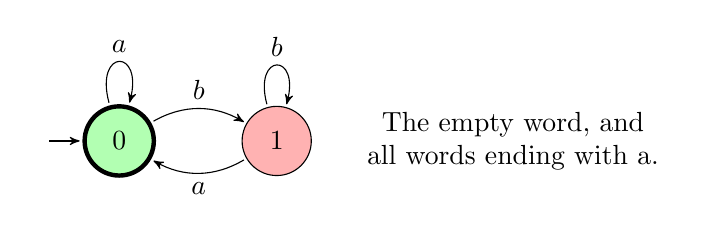
\begin{tikzpicture}
      \node[state, initial, accepting] (0)  {$0$};	
      \node[state, right of=0] (1)   {$1$};					
      
      \draw (0) edge[loop above]  node{$a$} (0);
      \draw (0) edge[bend left, above] node{$b$} (1);
      \draw (1) edge[bend left, below] node{$a$} (0);
      \draw (1) edge[loop above] node{$b$} (1);
      
      \node at (5,0) [text width=4cm, align=center] {The empty word, and all words ending with a.};
    \end{tikzpicture}
    \end{center}

    \begin{center}
      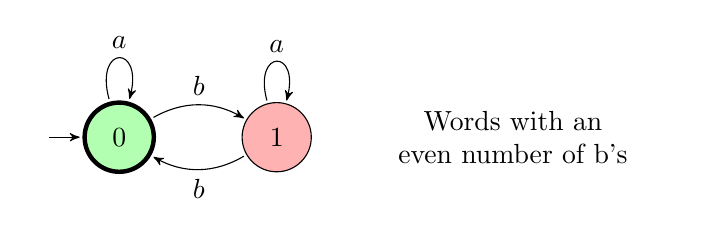
\begin{tikzpicture}
      \node[state, initial, accepting] (0)  {$0$};	
      \node[state, right of=0] (1)   {$1$};					
      
      \draw (0) edge[loop above]  node{$a$} (0);
      \draw (0) edge[bend left, above] node{$b$} (1);
      \draw (1) edge[bend left, below] node{$b$} (0);
      \draw (1) edge[loop above] node{$a$} (1);
      
      \node at (5,0) [text width=4cm, align=center] {Words with an even number of b's};
    \end{tikzpicture}
    \end{center}
    
    \begin{center}
      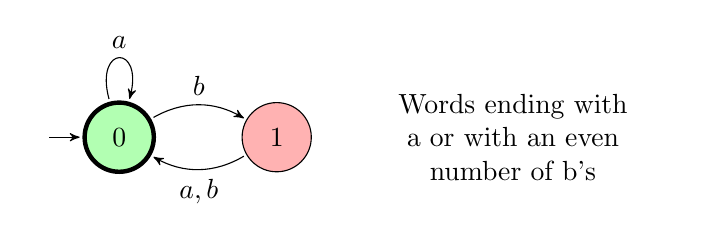
\begin{tikzpicture}
      \node[state, initial, accepting] (0)  {$0$};	
      \node[state, right of=0] (1)   {$1$};					
      
      \draw (0) edge[loop above]  node{$a$} (0);
      \draw (0) edge[bend left, above] node{$b$} (1);
      \draw (1) edge[bend left, below] node{$a, b$} (0);
      
      \node at (5,0) [text width=4cm, align=center] {Words ending with a or with an even number of b's};
    \end{tikzpicture}
    \end{center}
    \item If both $a$ and $b$ transition:
    \begin{center}
      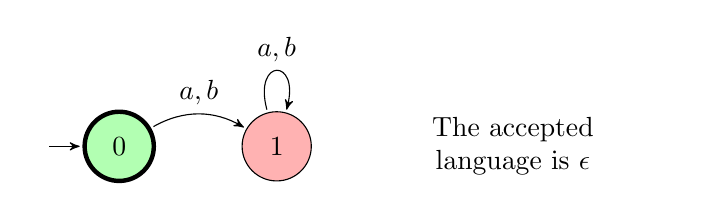
\begin{tikzpicture}
        \node[state, initial, accepting] (0) {$0$};
        \node[state, right of=0] (1) {$1$};
        
        \draw (0) edge[bend left, above] node{$a, b$} (1);
        \draw (1) edge[loop above] node{$a, b$} (1);
        
        \node at (5,0) [text width=4cm, align=center] {The accepted language is $\epsilon$};
    \end{tikzpicture}
    \end{center}

    \begin{center}
      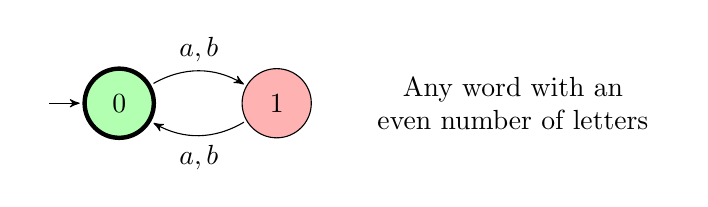
\begin{tikzpicture}
        \node[state, initial, accepting] (0) {$0$};
        \node[state, right of=0] (1) {$1$};
        
        \draw (0) edge[bend left, above] node{$a, b$} (1);
        \draw (1) edge[bend left, below] node{$a, b$} (0);
        
        \node at (5,0) [text width=4cm, align=center] {Any word with an even number of letters};
    \end{tikzpicture}
    \end{center}

    \begin{center}
      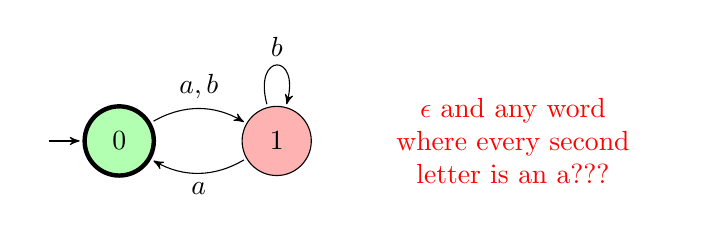
\begin{tikzpicture}
        \node[state, initial, accepting] (0) {$0$};
        \node[state, right of=0] (1) {$1$};
        
        \draw (0) edge[bend left, above] node{$a, b$} (1);
        \draw (1) edge[bend left, below] node{$a$} (0);
        \draw (1) edge[loop above] node{$b$} (1);
        
        \node at (5,0) [text width=4cm, align=center] {\textcolor{red}{$\epsilon$ and any word where every second letter is an a???}};
    \end{tikzpicture}
    \end{center}
  
  \end{itemize}
  
  \item \textit{A state in a DFA that is not accepting and all of those whose transitions are loops back to itself is sometimes called a "garbage state". Why?} \\
  $\to$ Because we can never leave that state to reach an accepting state.

  \item \textit{How many three state DFAs are there all of whose states are reachable and exactly one of which is a garbage state? What languages do they accept?}
  $\to$
\end{enumerate}

\subsubsection{Tutorial 02}
\begin{enumerate}
    \item \textit{If $\Sigma$ has $k$ elements how many different strings of length $n$ are there over $\Sigma$?} \\
    $\to$ There are $n^k$ possible strings.

    \item \textit{If $w \in \Sigma^*$ and $m, i + j \leq \left|w \right|$ how are:
    \begin{enumerate}
        \item the prefix of $w$ of length $m$,
        \item the suffix of $w$ of length $m$, and
        \item the substring of $w$ starting at position $i$ of length $j$
    \end{enumerate}
    defined?}\\
    Recall that $w$ is a function:
    $$
    w : \{0, 1, 2, \dots, n-1\} \to \Sigma
    $$
    \begin{enumerate}
        \item Prefix: 
        $$
         p : \{ 0, 1, \dots, m -1 \} \to \Sigma 
        $$
        $$
        p(i) = w(i)
        $$
        \item Suffix: 
        $$
         s : \{ 0, 1, \dots, m -1 \} \to \Sigma
        $$
        $$
        s(i) = w(i + n - m)
        $$
        \item Substring: 
        $$
         m : \{ 0, 1, \dots, j - 1 \} \to \Sigma
        $$
        $$
        m(t) = w(i + t)
        $$
    \end{enumerate}
    \item \textit{See S02.}
    \item \textit{Determine a regular grammar for the language of all strings containing an even number of a's (over $\Sigma = \{a, b\}$}
    \begin{align*}
        S \to & \epsilon \mid aO \mid bS \\
        O \to & aS \mid bO
    \end{align*}
    Basically, $S$ stands for ``even number of $a$'s so far" and $O$ for ``odd number of a's so far".

    \item \textit{Let \textbf{A} and \textbf{B} be DFAs over the same alphabet, $\Sigma$. Can you describe DFAs that accept:
    \begin{enumerate}
        \item The complement of the language $L(\textbf{A})$, i.e. the set of all strings not belonging to $L(\textbf{A})$.
        \item The intersection of $L(\textbf{A})$ and $L(\textbf{B})$, i.e. the set of all strings belonging to both of $L(\textbf{A})$ and $L(\textbf{B})$.
        \item The union of $L(\textbf{A})$ and $L(\textbf{B})$, i.e. the set of all strings belonging to at least one of $L(\textbf{A})$ and $L(\textbf{B})$.
    \end{enumerate}}
    $\to$ 
    \begin{enumerate}
        \item Interchange all the accepting and non-accepting states.
        \item For example, consider two automata: one that accepts strings with an even number of a's and any number of b's, and one that accepts strings with any number of a's and an even number of b's. Their  intersection is words with an even number of a's and b's. The ``cross product" machine is given on the website www.geeksforgeeks.org/cross-product-operation-in-dfa.com. The new machine will have 2 x 2 = 4 states.
        \item see the website.
    \end{enumerate}
    
    \item Repeat the previous question for the languages $L(\textbf{G})$ and $L(\textbf{H})$ associated to two \textit{right-regular grammars} over $\Sigma$.
    $\to$ In general, a right-regular grammar does not align exactly with a DFA (notably, the condition that state needs exactly one transition defined for each letter of the alphabet). In the case of the union, just list out the production rules. If any production rule leads back to the start symbol, we will be required to rename the start symbol for both machines.
    $$ s \rightarrow S_1 \mid S_2 $$
    Then include the production rules from both grammars.\\
    Because of the inherent non-determinism of grammars (where we might have multiple rules associated with a particular letter) it's not clear at all how one could realize the intersection of two languages or the complement of one.

\end{enumerate}

\end{document}